\documentclass[border=2pt]{standalone}
\usepackage{tikz}
\begin{document}
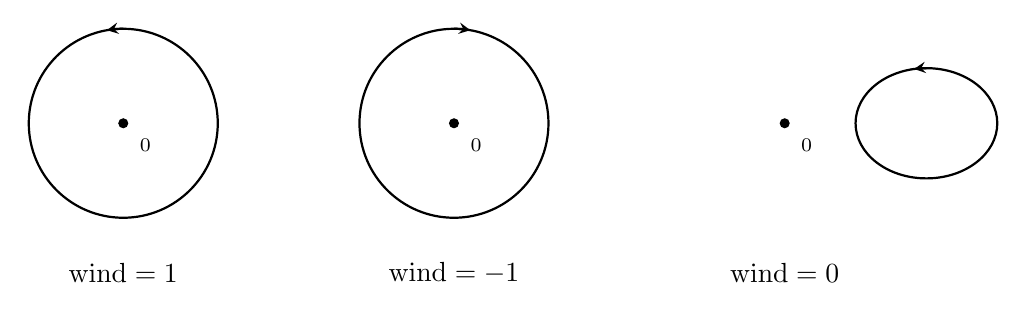
\begin{tikzpicture}[scale=1]
  % panel 1: wind = 1 (counterclockwise circle)
  \begin{scope}
    \draw[thick] (0,0) circle (1.2);
    \draw[thick,->,>=stealth] (0,1.2) arc (90:100:1.2);
    \filldraw (0,0) circle (1.6pt);
    \node at (0.28,-0.28) {\scriptsize $0$};
    \node at (0,-1.9) {${\rm wind}=1$};
  \end{scope}

  % panel 2: wind = -1 (clockwise circle)
  \begin{scope}[xshift=4.2cm]
    \draw[thick] (0,0) circle (1.2);
    \draw[thick,->,>=stealth] (0,1.2) arc (90:80:1.2);
    \filldraw (0,0) circle (1.6pt);
    \node at (0.28,-0.28) {\scriptsize $0$};
    \node at (0,-1.9) {${\rm wind}=-1$};
  \end{scope}

  % panel 3: wind = 0 (loop not enclosing the origin)
  \begin{scope}[xshift=8.4cm]
    \draw[thick] (1.8,0) ellipse (0.9 and 0.7);
    \draw[thick,->,>=stealth] (1.8,0.7) arc (90:100:0.9 and 0.7);
    \filldraw (0,0) circle (1.6pt);
    \node at (0.28,-0.28) {\scriptsize $0$};
    \node at (0,-1.9) {${\rm wind}=0$};
  \end{scope}
\end{tikzpicture}
\end{document}
